\documentclass[letterpaper,12pt]{article}
\usepackage{array}
\usepackage{threeparttable}
\usepackage{geometry}
\geometry{letterpaper,tmargin=1in,bmargin=1in,lmargin=1.25in,rmargin=1.25in}
\usepackage{fancyhdr,lastpage}
\pagestyle{fancy}
\lhead{}
\chead{}
\rhead{}
\lfoot{}
\cfoot{}
\rfoot{\footnotesize\textsl{Page \thepage\ of \pageref{LastPage}}}
\renewcommand\headrulewidth{0pt}
\renewcommand\footrulewidth{0pt}
\usepackage[format=hang,font=normalsize,labelfont=bf]{caption}
\usepackage{listings}
\lstset{frame=single,
	language=Python,
	showstringspaces=false,
	columns=flexible,
	basicstyle={\small\ttfamily},
	numbers=none,
	breaklines=true,
	breakatwhitespace=true
	tabsize=3
}
\usepackage{amsmath}
\usepackage{amssymb}
\usepackage{amsthm}
\usepackage{booktabs}
\usepackage{harvard}
\usepackage{setspace}
\usepackage{float,color}
\usepackage[pdftex]{graphicx}
\usepackage{hyperref}
\hypersetup{colorlinks,linkcolor=red,urlcolor=blue}
\theoremstyle{definition}
\newtheorem{theorem}{Theorem}
\newtheorem{acknowledgement}[theorem]{Acknowledgement}
\newtheorem{algorithm}[theorem]{Algorithm}
\newtheorem{axiom}[theorem]{Axiom}
\newtheorem{case}[theorem]{Case}
\newtheorem{claim}[theorem]{Claim}
\newtheorem{conclusion}[theorem]{Conclusion}
\newtheorem{condition}[theorem]{Condition}
\newtheorem{conjecture}[theorem]{Conjecture}
\newtheorem{corollary}[theorem]{Corollary}
\newtheorem{criterion}[theorem]{Criterion}
\newtheorem{definition}[theorem]{Definition}
\newtheorem{derivation}{Derivation} % Number derivations on their own
\newtheorem{example}[theorem]{Example}
\newtheorem{exercise}[theorem]{Exercise}
\newtheorem{lemma}[theorem]{Lemma}
\newtheorem{notation}[theorem]{Notation}
\newtheorem{problem}[theorem]{Problem}
\newtheorem{proposition}{Proposition} % Number propositions on their own
\newtheorem{remark}[theorem]{Remark}
\newtheorem{solution}[theorem]{Solution}
\newtheorem{summary}[theorem]{Summary}
%\numberwithin{equation}{section}
\bibliographystyle{aer}
\newcommand\ve{\varepsilon}
\newcommand\boldline{\arrayrulewidth{1pt}\hline}
\usepackage{graphicx}   % already in your preamble
\raggedright


\begin{document}
	
	\begin{center}
		\textbf{\large{Problem Set 5}} \\
	\end{center}
	
	\begin{flushleft}
		ECON833, Prof. Jason DeBacker \\
		Gyumin Kim
	\end{flushleft}
	
	\vspace{5mm}
	
	\textbf{Part A: Visualization} 
		\textbf{Research Question and description}
     Stockout-based size spillover effects refer to the sales of adjacent size products increases when focal product size is out-of-stock. For example, when jeans with size of 30 is out-of-stock, the sales of jeans with size of 31 or 29 increases. I will only identify the bigger size spillover effects of jeans because smaller size jeans are less likely to be chosen as an alternative option for customer facing out-of-stock of their most preferred size. Moreover, I will show this effect is positively moderated by the fitting room visits of treatment products. 	 \vspace{1mm}
     
    
    I want to investigate the relationship between stockout-based size spillover effects and the fitting room visits of jeans. Because jeans are the products which are the most frequently brought into the fitting rooms. Before identifying this relationship, I will show whether the stockout-based size spillover effects exist in the case of jeans. 
    
     	\textbf{Data description}
     	
     I obtained the data from Korean fast fashion brand. You can easily think of Korean version Zara. I have inventory, transaction and fitting room data for this brand. What I received is dataset merged of three datasets including only jeans. Therefore, I clean my data and create variables needed to run my model. 
     
     Inventory data captures when stock level of the specific products and transaction data captures transaction of the specific products enabling me to obtain sales variable. Fitting room data is unique. This captures whether and when the specific products are brought into the fitting rooms.\vspace{1mm}
     
     I include OOS, treatment, fit, age, price variables in my models. OOS is indicator variable showing the status of out-of-stock of focal products. If focal product is out-of-stock in the day t, I assigned OOS = 1, otherwise 0. Treatment is 1 when focal product is out of stock, the one size bigger product of focal product which is out-of-stock in day t is assigned as treatment group,while Treatment is 0 when focal product is out of stock, the two size bigger product of focal product which is out-of-stock in day t is assigned as control. fit represents the number of fitting room visits for product and price is the retail price for product.  Age stands for the age of products calculated by the day elapsed from product's launch date and the day t.      \vspace{1mm}
     
     I assigned adjacent size product which means that one size bigger jeans as treatment group. Control groups consists of two size bigger jeans when the focal size products are out-of-stock. I compare the log sales of before and after the stockouts for focal size product with both treatment and control groups. 
		
	\begin{figure}[H]
		\centering
		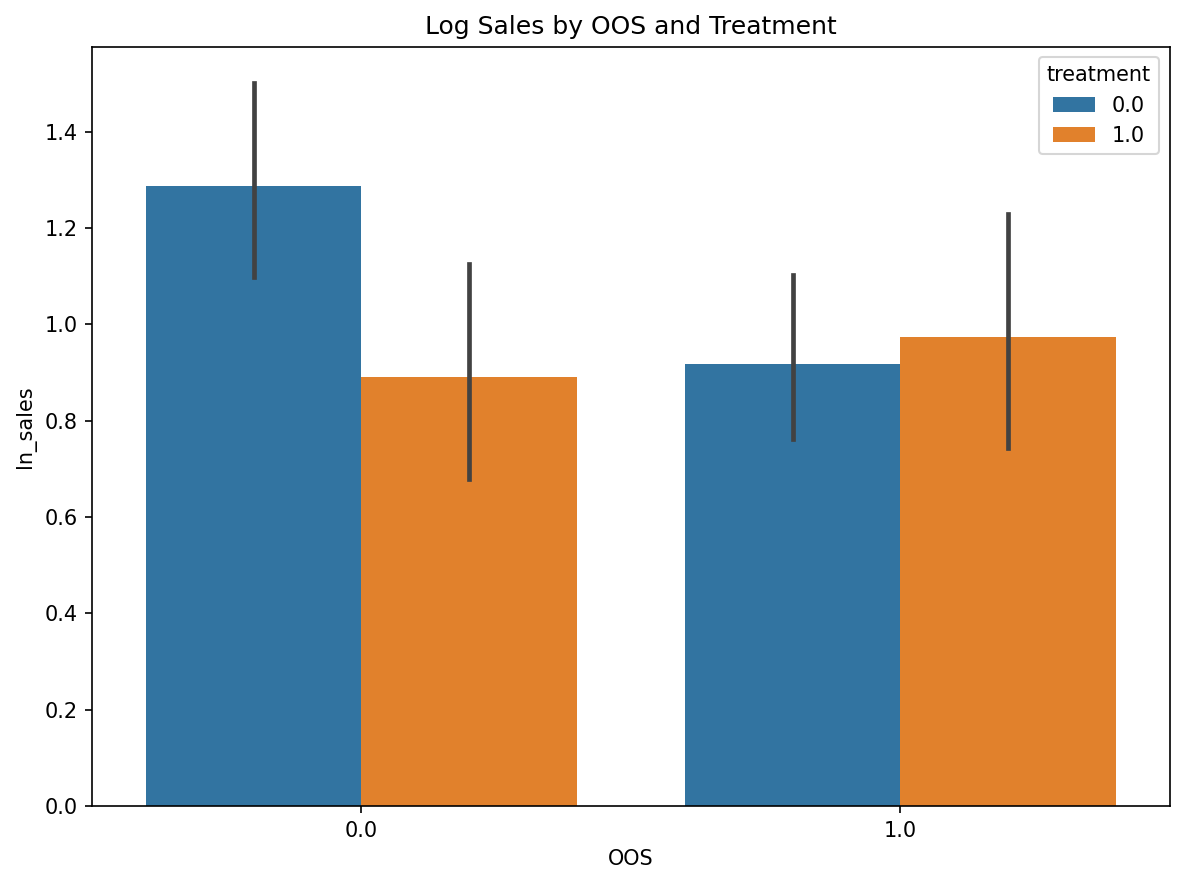
\includegraphics[width=0.7\textwidth]{images/LogSales.png}
		\caption{}
		\label{Log Sales by Treatment Group}
	\end{figure}
	
	As you can see from Figure 1, while the sales of both treatment groups and control group before the focal products are out-of-stock are different, the sales of treatment group and control group after the stockouts of focal products are relatively identical. 
	
	From now, I will compare the number of fitting room visits of jeans of before and after the stockouts for focal size product with treatment group and control group.	
	
	\begin{figure}[H]
		\centering
		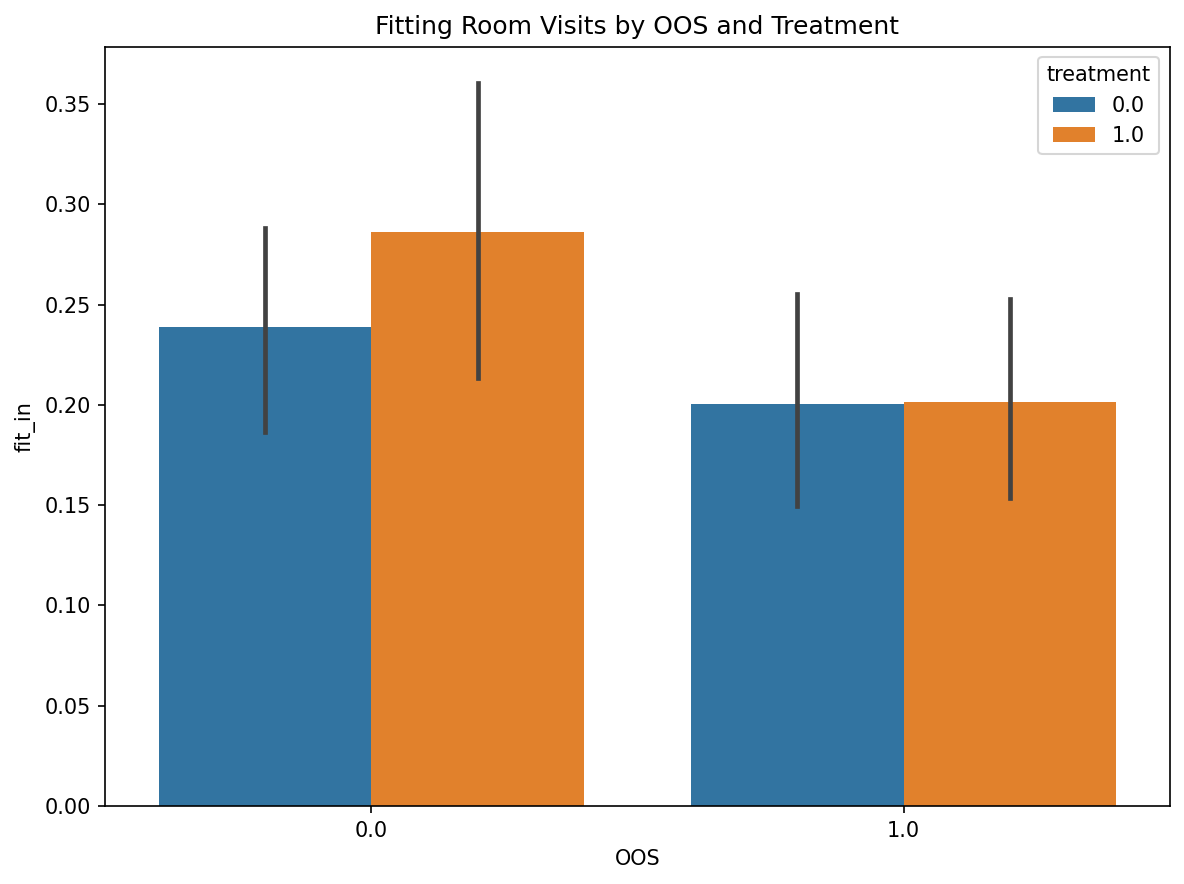
\includegraphics[width=0.7\textwidth]{images/Fittingroomvisits.png}
		\caption{}
		\label{Fittingroom visits}
	\end{figure}
	
	In this histogram, it is hard to see that there is a significant difference in fitting room visits of jeans between treatment group and control group after the focal products are stockout. However, what I want to know is whether the sales of adjacent size of jeans increases as the fitting room visits of adjacent size of jeans increase. This requires me to utilize Difference-in-Difference-in-Differences (DDD) methods.
	
	Before I ran a Difference-in-Differences (DID) regression, one assumption that I have to confirm is pre-parallel trend assumption. In this situation, pre-period stands for in-stock period of focal jeans. Therefore, I want to visualize the sales trend of one size bigger jeans(treatment group) and two size bigger jeans(control group) and compare them to identify whether they have parallel trend in sales. 
	
	\begin{figure}[H]
		\centering
		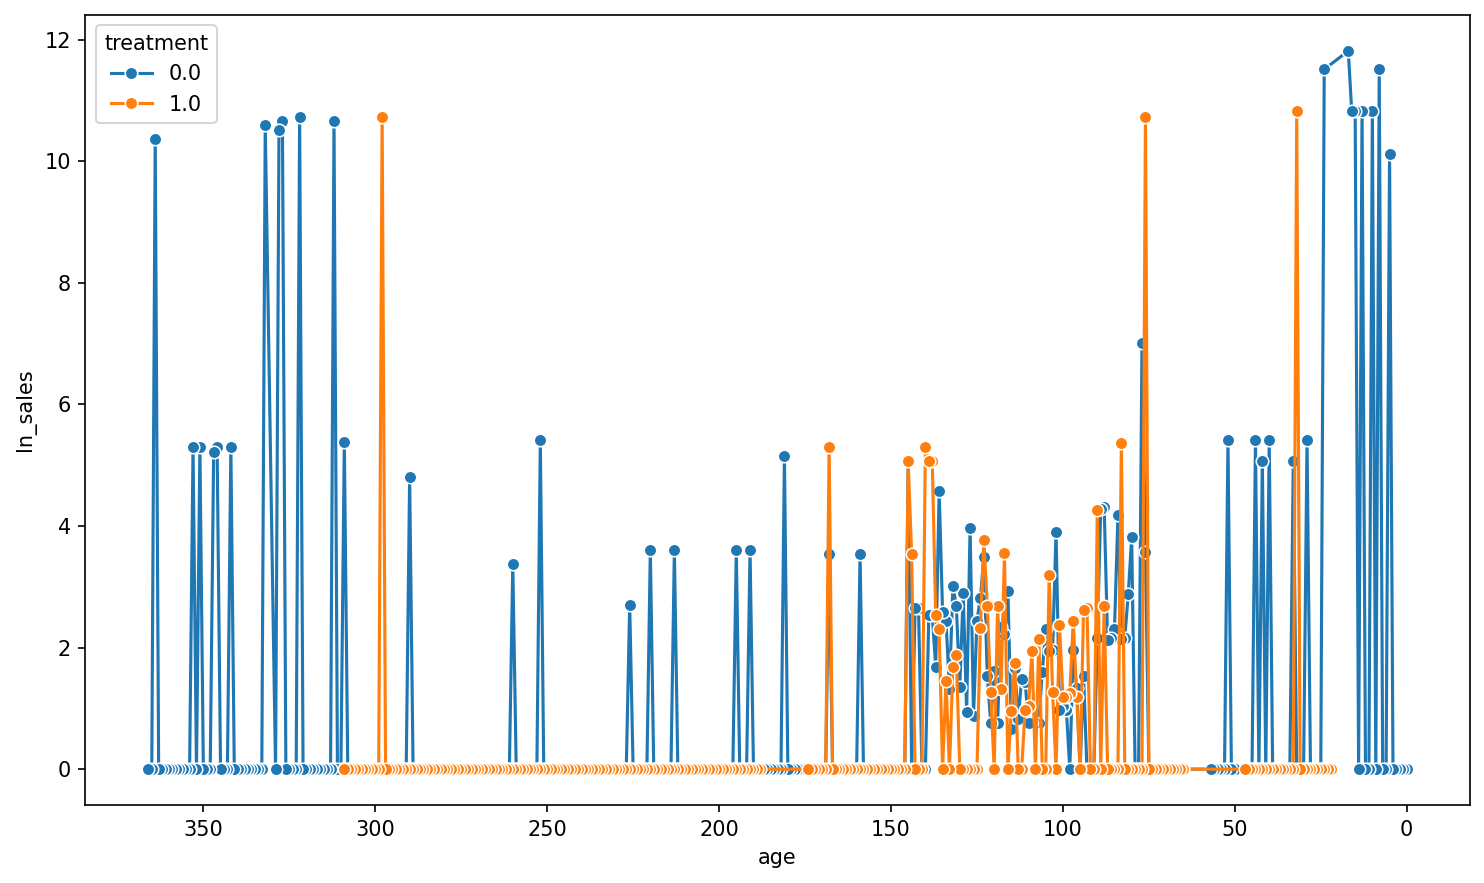
\includegraphics[width=0.7\textwidth]{images/SalesTrend.png}
		\caption{}
		\label{SalesTrend}
	\end{figure}
	
	As we can see from the Figure 3, the sales trend of treatment and control groups are almost identical between 150 and 50. Therefore, I can argue that there is no reason for attributing the sales increase to other unobserved time-variant factors. 
	However, it is hard to say that there is a parallel tern before 150 days and after 50 days. 
	I have to delve into this more later.  
	
	 
	 \vspace{5mm}
	 
	 \textbf{Part B: Econometric Models} 
	 
\begin{table}[htbp]
\centering
\begin{tabular}{lrrr}
\toprule
 & DID & 3-way & Treat×Age \\
\midrule
C(OOS)[T.1.0] & -0.365** & -0.373** &  \\
C(OOS)[T.1.0] (se) & (0.181) & (0.178) &  \\
C(OOS)[T.1.0]:fit\_in &  & 0.031 &  \\
C(OOS)[T.1.0]:fit\_in (se) &  & (0.259) &  \\
C(treatment)[T.1.0] & 0.248 & 0.218 & 0.299 \\
C(treatment)[T.1.0] (se) & (0.200) & (0.249) & (0.412) \\
C(treatment)[T.1.0]:C(OOS)[T.1.0] & 0.548** & 0.418 &  \\
C(treatment)[T.1.0]:C(OOS)[T.1.0] (se) & (0.264) & (0.259) &  \\
C(treatment)[T.1.0]:C(OOS)[T.1.0]:fit\_in &  & 0.692* &  \\
C(treatment)[T.1.0]:C(OOS)[T.1.0]:fit\_in (se) &  & (0.410) &  \\
C(treatment)[T.1.0]:age &  &  & -0.002 \\
C(treatment)[T.1.0]:age (se) &  &  & (0.003) \\
C(treatment)[T.1.0]:fit\_in &  & 0.104 &  \\
C(treatment)[T.1.0]:fit\_in (se) &  & (0.359) &  \\
age & -0.011 & -0.016 & -0.051* \\
age (se) & (0.016) & (0.016) & (0.027) \\
fit\_in & 1.210*** & 1.102*** & 1.146*** \\
fit\_in (se) & (0.191) & (0.286) & (0.218) \\
price & 0.000 & 0.000 & 0.000* \\
price (se) & (0.000) & (0.000) & (0.000) \\
Observations & 3589 & 3589 & 1843 \\
R-squared & 0.189 & 0.194 & 0.225 \\
\bottomrule
\end{tabular}

\caption{Selected coefficients}
\label{tab:selected_models}
\end{table}


 This table shows the results from DID, DDD, and pre-parallel trend assumption tests. 
 
  \vspace{1mm}
  
  First column presents the results of interaction term between treatment and OOS. As you can see the coefficient is positive and significant. Because the dependent variable is log sales, we can interpret that after focal products are out-of-stock, the sales of one size bigger product increase about 54 percent, which is pretty huge amount. 
  
   \vspace{1mm}
   
   Second column demonstrates that this stockout-based bigger size spillover effects is strengthened as the treatment product is brought into the fitting rooms. As you can see in the table, positive but weakly significant is obtained. We can argue conservatively that this effect is positively moderated by the number of fitting room visits. 
   
    
   \vspace{1mm}
   
   Third column explains that pre-parallel trend is supported. In DID setting, It is important to validate pre-parallel trend assumption to prove that increase is not attributed to unobserved time varying factors. Therefore, I ran DID regression with interaction term between treatment variable and age variable before the focal product is out-of-stock. While I obtain insignificant result of interaction term between age and treatment, I have to delve into this more because the graph that I have shown before seems problematic. 




	 
	  
\end{document}   